\section{信号与无线信道}

\subsection{信号的本质}

我们每天都在与信号打交道。当你说话时，声波在空气中传播；当你打开手机，电磁波在空间中穿行。但这两种信号有着本质的区别。

声波是纵波，它的振动方向与传播方向相同，依靠空气分子的疏密变化来传递能量。这也是为什么声波无法在真空中传播——没有介质，就没有可以振动的分子。但电磁波不同，它是横波，电场与磁场的振动方向都与传播方向垂直，且互相垂直。这种结构使电磁波可以在真空中传播，速度达到每秒30万公里，远超声波在空气中的344米每秒。

\begin{figure}[htbp]
    \centering
    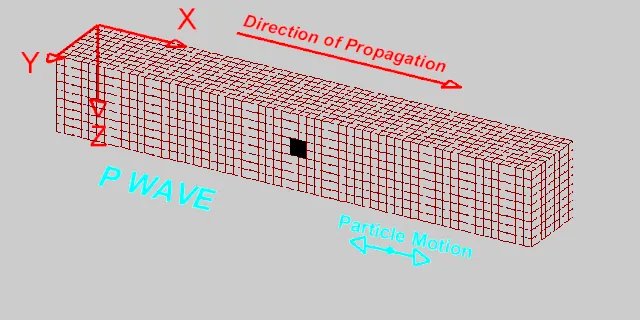
\includegraphics[width=0.7\textwidth]{assets/ch02/ch02-2_3_信号-000.png}
    \caption{纵波（P波）传播示意图：质点振动方向与波传播方向相同}
    \label{fig:p-wave}
\end{figure}

这一物理特性决定了无线通信的可能。但自由传播的代价是信道环境的不可控性——与封闭的导线不同，无线信号要穿越开放空间，遭遇各种障碍和干扰。理解这些特性，是设计无线通信系统的起点。

\subsection{正弦波与信号的基本参数}

最简单的信号是正弦波。虽然它看似简单，但任何复杂的周期信号都可以分解为正弦波的叠加。正弦波的数学表达式为
\begin{equation}
    s(t) = A \sin(2\pi f t + \phi)
\end{equation}
其中 $A$ 是振幅，表示信号的强度；$f$ 是频率，单位为赫兹（Hz），表示每秒振动的次数；$\phi$ 是相位，表示信号在时间轴上的起始位置。周期 $T$ 与频率互为倒数，$T = 1/f$；波长 $\lambda$ 则是一个周期占据的空间长度，$\lambda = vT$，其中 $v$ 是传播速度。

\begin{figure}[htbp]
    \centering
    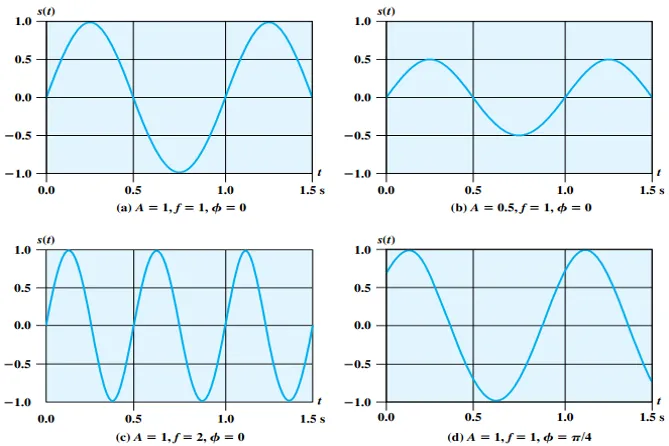
\includegraphics[width=0.9\textwidth]{assets/ch02/ch02-2_3_信号-003.png}
    \caption{正弦波的参数变化：振幅、频率和相位对波形的影响}
    \label{fig:sine-parameters}
\end{figure}

振幅与频率的物理意义直观可感。弹吉他时，用力拨弦会增大振幅，声音更响亮；使用更细的弦会提高振动频率，音调更高。人耳可感知的声波频率范围约为20 Hz到20 kHz。电话系统为了节省带宽，通常只传输300到3400 Hz的范围；高保真音响则追求20 Hz到20 kHz的全频带还原。

\subsection{傅里叶分析：从时域到频域}

实际通信中的信号远比正弦波复杂。但1768年出生的法国数学家傅里叶发现，任何周期信号都可以表示为正弦波的和。这一发现成为信号分析的基石。

考虑一个周期为 $T$ 的信号 $s(t)$，满足 $s(t) = s(t+T)$。傅里叶证明了，这个信号可以写成
\begin{equation}
    s(t) = a_0 + \sum_{n=1}^{\infty} \left( a_n \cos \frac{2\pi n t}{T} + b_n \sin \frac{2\pi n t}{T} \right)
\end{equation}
这就是傅里叶级数。其中 $a_0$ 是直流分量，$n=1$ 的项是基频分量，$n>1$ 的项是谐波分量。

\begin{figure}[htbp]
    \centering
    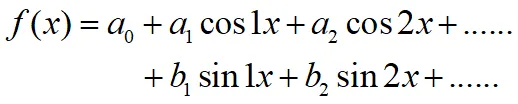
\includegraphics[width=0.6\textwidth]{assets/ch02/ch02-2_3_信号-009.png}
    \caption{周期信号的傅里叶级数展开：任意周期信号可表示为正弦/余弦波的叠加}
    \label{fig:fourier-series}
\end{figure}

现在的问题是：如何确定这些系数 $a_n$ 和 $b_n$？

\subsubsection{正交性的核心作用}

求解系数的关键在于三角函数的\textbf{正交性}。正交原本是几何概念，指两个矢量成直角。函数的正交性与此类似：如果两个函数在一个周期内的乘积积分为零，就称它们正交。

正弦和余弦函数具有优美的正交性质。在 $[0, 2\pi]$ 区间内，$\sin x$ 与 $\cos x$ 正交，因为它们相差 $\pi/2$ 的相位——在圆周上正好是90度。更一般地，不同频率的正弦函数互相正交，相同频率的正弦和余弦也正交。

\begin{figure}[htbp]
    \centering
    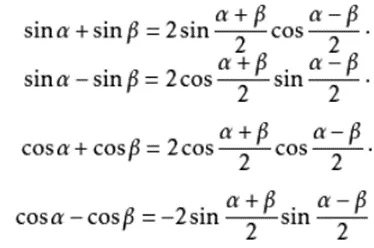
\includegraphics[width=0.5\textwidth]{assets/ch02/ch02-2_3_信号-013.png}
    \caption{三角函数积化和差公式：用于验证正交性关系}
    \label{fig:trig-formulas}
\end{figure}

具体而言，对于整数 $m, n$：
\begin{align}
    \int_0^{2\pi} \sin(mx) \cos(nx) \, dx &= 0 \quad \text{（对所有 $m, n$）} \\
    \int_0^{2\pi} \sin(mx) \sin(nx) \, dx &= \begin{cases} \pi, & m = n \neq 0 \\ 0, & m \neq n \end{cases} \\
    \int_0^{2\pi} \cos(mx) \cos(nx) \, dx &= \begin{cases} \pi, & m = n \neq 0 \\ 2\pi, & m = n = 0 \\ 0, & m \neq n \end{cases}
\end{align}

这些等式可以通过三角函数的积化和差公式证明，但它们的意义更为深远：正交性使我们能够"提取"信号中特定频率的成分。

\subsubsection{系数求解的推导}

利用正交性，我们可以逐一确定傅里叶系数。以求 $b_n$（正弦分量的系数）为例，将傅里叶级数两边乘以 $\sin(nx)$ 并在 $[0, 2\pi]$ 上积分：
\begin{equation}
    \int_0^{2\pi} s(x) \sin(nx) \, dx = \int_0^{2\pi} \left[ a_0 + \sum_{m=1}^{\infty} (a_m \cos(mx) + b_m \sin(mx)) \right] \sin(nx) \, dx
\end{equation}

根据正交性，右边只剩下 $m=n$ 的正弦项：
\begin{equation}
    \int_0^{2\pi} s(x) \sin(nx) \, dx = b_n \int_0^{2\pi} \sin^2(nx) \, dx = b_n \cdot \pi
\end{equation}

因此
\begin{equation}
    b_n = \frac{1}{\pi} \int_0^{2\pi} s(x) \sin(nx) \, dx
\end{equation}

同理，对于余弦系数：
\begin{equation}
    a_n = \frac{1}{\pi} \int_0^{2\pi} s(x) \cos(nx) \, dx \quad (n \geq 1)
\end{equation}

直流分量 $a_0$ 稍有不同，因为 $\cos(0) = 1$ 的积分范数是 $2\pi$：
\begin{equation}
    a_0 = \frac{1}{2\pi} \int_0^{2\pi} s(x) \, dx
\end{equation}

这就是傅里叶系数的完整表达式。它们告诉我们：任何周期信号都由一个直流分量和一系列正弦、余弦谐波组成，各分量的强度由上述积分确定。

\subsubsection{指数形式的统一表达}

傅里叶级数还可以写成更紧凑的指数形式。利用欧拉公式 $e^{j\theta} = \cos\theta + j\sin\theta$，可以验证三角级数与指数级数的等价性。

定义复系数
\begin{equation}
    c_n = \frac{1}{2\pi} \int_0^{2\pi} s(x) e^{-jnx} \, dx
\end{equation}

则信号表示为
\begin{equation}
    s(t) = \sum_{n=-\infty}^{\infty} c_n e^{jnt}
\end{equation}

这种形式在计算上更为简洁，也便于推广到非周期信号的傅里叶变换。

\begin{figure}[htbp]
    \centering
    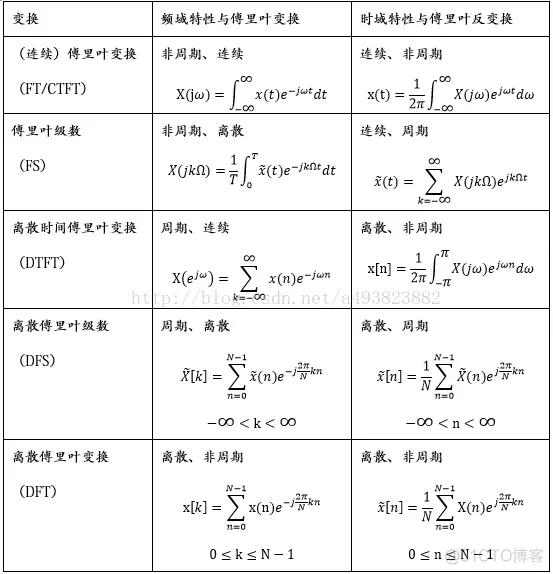
\includegraphics[width=0.9\textwidth]{assets/ch02/ch02-2_3_信号-028.png}
    \caption{五种傅里叶变换形式的对照表：时域与频域特性的对应关系}
    \label{fig:fourier-transforms}
\end{figure}

\subsection{信号的能量与功率}

信号的能量和功率是衡量信号强度的基本指标。能量定义为信号平方的积分
\begin{equation}
    E = \int_{-\infty}^{\infty} |x(t)|^2 dt
\end{equation}

对于周期信号，能量无限，因此定义平均功率更有意义
\begin{equation}
    P = \frac{1}{T_0} \int_0^{T_0} |x(t)|^2 dt
\end{equation}

这里有一个深刻的结果。将周期信号的傅里叶级数代入功率表达式，利用正交性，得到
\begin{equation}
    P = |a_0|^2 + \frac{1}{2} \sum_{n=1}^{\infty} (|a_n|^2 + |b_n|^2) = \sum_{n=-\infty}^{\infty} |c_n|^2
\end{equation}

这就是\textbf{帕塞瓦尔定理}：信号的时域功率等于其各频率分量功率之和。它表明能量在时域和频域的分布是等价的。

\begin{figure}[htbp]
    \centering
    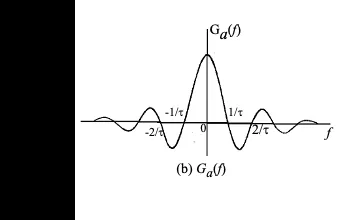
\includegraphics[width=0.4\textwidth]{assets/ch02/ch02-2_3_信号-032.png}
    \caption{功率谱密度定义：信号功率在频域的分布}
    \label{fig:psd}
\end{figure}

\subsection{无线信道的挑战}

有线通信中，信号被限制在导线内，环境相对可控。无线通信面对的是开放空间，信号在传播过程中遭遇多种损伤。

\subsubsection{路径损耗与距离的较量}

最基本的损伤是路径损耗——信号随距离增加而衰减。自由空间模型给出了理论基准
\begin{equation}
    P_r = P_t \cdot G_t \cdot G_r \cdot \left(\frac{\lambda}{4\pi d}\right)^2
\end{equation}

其中 $P_t$ 和 $P_r$ 分别是发射和接收功率，$G_t$ 和 $G_r$ 是天线增益，$\lambda$ 是波长，$d$ 是距离。这个公式揭示了两个重要事实：接收功率与距离的平方成反比，与波长的平方成正比。高频信号（短波长）比低频信号衰减更快。

但真实环境远比自由空间复杂。城市中的建筑物、山丘、植被都会阻挡信号。这种阻挡是随机的——你无法精确预测某一具体位置的遮挡程度，但可以用统计模型描述。研究者发现，考虑这些障碍物的综合效应后，信号衰减服从对数正态分布。对数距离路径损耗模型将确定性衰减和随机阴影结合
\begin{equation}
    PL(d) = PL(d_0) + 10n \log_{10}\left(\frac{d}{d_0}\right) + X_\sigma
\end{equation}
其中 $n$ 是路径损耗指数，自由空间 $n=2$，城市环境可达 $3.7$ 到 $6.5$；$X_\sigma$ 是零均值高斯随机变量，代表阴影衰落的随机性。

\subsubsection{多径效应与小尺度衰落}

比阴影更复杂的是多径效应。无线信号从发射端到接收端，可能经历反射、折射、散射和绕射，通过多条路径到达。这些路径长度不同，信号副本以不同相位叠加，导致接收信号强度的快速波动。

多径信道可以用时变冲激响应描述
\begin{equation}
    h(t, \tau) = \sum_{i=1}^{N(t)} a_i(t) e^{-j\phi_i(t)} \delta(\tau - \tau_i(t))
\end{equation}
其中 $a_i$ 是第 $i$ 条路径的幅度，$\tau_i$ 是时延，$\phi_i$ 是相位，$N$ 是多径数量。

由此引出几个关键参数。时延扩展 $T_m$ 是最大多径时延差，它决定了信道是否频率选择性——如果信号带宽远大于 $1/T_m$，不同频率会经历不同衰落。相干带宽 $B_c \approx 1/T_m$ 是信道响应近似恒定的频率范围。

类似地，移动导致的多普勒效应使信道随时间变化。多普勒扩展 $f_D = v/\lambda$ 衡量这种变化的速度，相干时间 $T_c \approx 1/f_D$ 是信道近似不变的时间窗口。

\subsubsection{衰落的统计模型}

当没有直射路径且多径丰富时，接收信号包络服从\textbf{瑞利分布}
\begin{equation}
    f_R(r) = \frac{r}{\sigma^2} e^{-r^2/(2\sigma^2)}, \quad r \geq 0
\end{equation}
这是大量独立多径分量的矢量和的结果。根据中心极限定理，同相和正交分量都服从高斯分布，其包络即为瑞利分布。

当存在直射路径时，信号包含一个稳定分量叠加随机多径，此时包络服从\textbf{莱斯分布}
\begin{equation}
    f_R(r) = \frac{r}{\sigma^2} e^{-(r^2+K^2)/(2\sigma^2)} I_0\left(\frac{rK}{\sigma^2}\right)
\end{equation}
其中 $K$ 是莱斯因子，表示直射分量与散射分量的功率比。$K$ 越大，信道越稳定，越接近AWGN信道；$K$ 越小，越接近瑞利衰落。

\subsubsection{噪声的物理起源}

无线信道中不可避免的干扰是噪声。热噪声源于导体中电子的热运动，其功率谱密度为 $N_0 = kT$，其中 $k$ 是玻尔兹曼常数，$T$ 是绝对温度。在带宽 $B$ 内的噪声功率为 $N = kTB$。

热噪声被建模为\textbf{加性高斯白噪声}（AWGN）。"加性"表示噪声独立叠加于信号；"高斯"表示幅度服从高斯分布；"白"表示功率谱密度在所有频率上为常数。AWGN是通信系统分析的标准模型，实际系统的性能最终都受限于这一物理噪声。

信噪比 $\text{SNR} = S/N$ 是信号功率与噪声功率之比，是决定通信质量的关键参数。提高发射功率可以增加SNR，但受限于法规和设备能力；降低噪声需要更先进的低噪声放大器或更冷的接收机——后者在深空通信中确实被采用。

\subsection{从傅里叶到拉普拉斯：为什么要推广}

傅里叶分析提供了观察信号的频域视角，但它有一个根本性的限制——要求信号满足绝对可积条件。许多实际信号并不满足这一条件：阶跃信号在无穷远处不衰减，指数增长的信号能量无限，这些信号在严格意义上没有傅里叶变换。

更重要的是，傅里叶变换无法直接处理系统的因果性。当我们分析一个从某一时刻启动的电路，或研究一个从静止开始运动的机械系统，初始条件如何纳入分析框架？系统的瞬态响应如何与稳态特性统一描述？

拉普拉斯变换正是为解决这些问题而生。它通过引入一个指数衰减因子 $e^{-\sigma t}$，将原本不收敛的信号转化为可变换的形式，同时将微分方程转化为代数方程，将初始条件自然地嵌入变换域。

\subsubsection{收敛性与衰减因子}

考虑一个简单的问题：单位阶跃信号 $u(t)$ 在 $t \geq 0$ 时恒为1，它的傅里叶变换存在吗？从定义出发
\begin{equation}
    \int_{-\infty}^{\infty} u(t) e^{-j\omega t} dt = \int_{0}^{\infty} e^{-j\omega t} dt
\end{equation}
这个积分不收敛，因为被积函数在 $t \to \infty$ 时不趋于零。但如果我们乘以一个衰减因子 $e^{-\sigma t}$，其中 $\sigma > 0$
\begin{equation}
    \int_{0}^{\infty} e^{-\sigma t} e^{-j\omega t} dt = \int_{0}^{\infty} e^{-(\sigma + j\omega)t} dt = \frac{1}{\sigma + j\omega}
\end{equation}
积分收敛了。这个观察引向关键的推广：将频率从实轴扩展到复平面。

定义复频率 $s = \sigma + j\omega$，其中 $\sigma$ 是实部，控制衰减或增长；$\omega$ 是虚部，代表角频率。信号 $x(t)$ 的双边拉普拉斯变换定义为
\begin{equation}
    X(s) = \int_{-\infty}^{\infty} x(t) e^{-st} dt
\end{equation}

当 $\sigma = 0$ 时，$s = j\omega$，拉普拉斯变换退化为傅里叶变换。这意味着傅里叶变换是拉普拉斯变换在虚轴上的特例。拉普拉斯变换将频域分析推广到整个复平面，大大扩展了可分析信号的范围。

\subsubsection{单边变换与因果系统}

实际系统通常是因果的——响应不会早于激励发生。对于因果信号 $x(t) = 0$（当 $t < 0$），单边拉普拉斯变换更为适用
\begin{equation}
    X(s) = \int_{0^-}^{\infty} x(t) e^{-st} dt
\end{equation}
积分下限 $0^-$ 包含了 $t=0$ 时刻可能存在的冲激，确保初始条件被完整捕获。

单边变换的真正威力体现在微分性质上。考虑 $x(t)$ 的导数的变换
\begin{equation}
    \mathcal{L}\left\{\frac{dx}{dt}\right\} = \int_{0^-}^{\infty} \frac{dx}{dt} e^{-st} dt
\end{equation}
分部积分得到
\begin{equation}
    \mathcal{L}\left\{\frac{dx}{dt}\right\} = sX(s) - x(0^-)
\end{equation}
导数运算变成了乘以 $s$ 并减去初始值。这一性质将时域微分方程转化为变换域的代数方程，初始条件 $x(0^-)$ 自然地出现在方程中。

\subsubsection{系统分析与传递函数}

线性时不变系统由冲激响应 $h(t)$ 完全刻画。输入 $x(t)$ 产生的输出是卷积 $y(t) = x(t) * h(t)$。在拉普拉斯域，卷积变为乘积
\begin{equation}
    Y(s) = X(s) H(s)
\end{equation}
其中 $H(s)$ 是系统的传递函数，是冲激响应的拉普拉斯变换。

传递函数提供了系统分析的强大工具。系统的极点（使 $H(s)$ 分母为零的 $s$ 值）决定了系统的固有响应模式。实极点对应指数衰减或增长，共轭复极点对应衰减或增长的正弦振荡。极点的位置揭示了系统的稳定性：所有极点位于左半平面时，系统稳定；存在右半平面极点时，系统不稳定。

零点（使 $H(s)$ 分子为零的 $s$ 值）则影响系统的频率选择特性。极零点在复平面上的配置完全刻画了系统的输入输出行为，这是控制系统设计的几何语言。

\subsubsection{从连续到离散：Z变换的引入}

数字信号处理将连续时间信号采样为离散序列。采样间隔 $T$ 将连续时间 $t$ 映射为离散序号 $n$，信号 $x(t)$ 变为序列 $x[n] = x(nT)$。

对离散序列直接应用拉普拉斯变换，令 $t = nT$
\begin{equation}
    X(s) = \sum_{n=-\infty}^{\infty} x[n] e^{-snT}
\end{equation}
定义 $z = e^{sT}$，则 $e^{-snT} = z^{-n}$，得到Z变换的定义
\begin{equation}
    X(z) = \sum_{n=-\infty}^{\infty} x[n] z^{-n}
\end{equation}

Z变换与拉普拉斯变换通过 $z = e^{sT}$ 关联。复 $s$ 平面的虚轴映射到 $z$ 平面的单位圆，左半平面映射到单位圆内部，右半平面映射到单位圆外部。稳定系统的极点必须位于单位圆内。

\subsubsection{Z变换的性质与系统分析}

Z变换继承了拉普拉斯变换的核心优点，并适应了离散时间特性。时移性质尤为简洁：序列右移一位对应乘以 $z^{-1}$
\begin{equation}
    \mathcal{Z}\{x[n-1]\} = z^{-1} X(z)
\end{equation}
$z^{-1}$ 因此被称为单位延迟算子，它是数字滤波器实现的基本构件。

差分方程描述离散时间系统，类似于连续时间的微分方程。Z变换将差分方程转化为代数方程。考虑一阶差分方程
\begin{equation}
    y[n] + a y[n-1] = b x[n]
\end{equation}
Z变换后得到
\begin{equation}
    Y(z) + a z^{-1} Y(z) = b X(z)
\end{equation}
传递函数为
\begin{equation}
    H(z) = \frac{Y(z)}{X(z)} = \frac{b}{1 + a z^{-1}} = \frac{b z}{z + a}
\end{equation}
极点位于 $z = -a$。当 $|a| < 1$ 时极点在单位圆内，系统稳定。这一判据比连续时间系统更直观——只需检查极点是否在单位圆内。

\subsubsection{三种变换的统一视角}

傅里叶变换、拉普拉斯变换和Z变换构成了信号分析的三层框架。傅里叶变换分析信号的频谱组成，适用于稳态、能量有限的信号。拉普拉斯变换扩展了分析范围，引入衰减因子处理增长信号，自然纳入初始条件，统一描述瞬态和稳态响应。Z变换将这一框架移植到离散时间领域，为数字信号处理提供数学基础。

三者的关系通过极限和映射体现。拉普拉斯变换在虚轴上退化为傅里叶变换；Z变换通过 $z = e^{sT}$ 与拉普拉斯变换关联，当采样间隔 $T \to 0$ 时，Z变换趋近拉普拉斯变换。这一层次结构使工程师能够在不同域中选择最适合的分析工具，而它们之间的深刻联系确保了理论的一致性和完整性。

在通信系统设计中，这些变换各有用武之地。模拟滤波器设计在拉普拉斯域进行，通过极零点配置实现所需的频率响应。数字滤波器在Z域设计，通过差分方程实现。系统级仿真则在频域进行，利用傅里叶变换的快速算法计算信号通过线性系统的响应。掌握这三种变换及其相互关系，是深入理解信号处理与通信系统的关键。
